\section{Agile - I Lecture}

\subsection{Introduction}

Welcome to this ten-hour course where I will guide you through the
objectives, my background, and the three main topics we will cover.
Throughout this course, we will explore basic concepts of Agile and
Methodologies, Microservices Architectures, and DevOps techniques.
Please note that the goal of this course is not to make you an expert in
these areas, but rather to provide you with a solid understanding of the
fundamentals. Let's dive in!

\subsection{Topics Overview}

\subsubsection{Agile Methodologies}

My main objective is to provide you with a vocabulary that you can share
and use when discussing these topics with experts. By understanding
these concepts, you will be able to engage in meaningful conversations
with others. Now, let's dive into the topics.

\begin{figure}[!h]
  \centering
  \includegraphics[page=3, trim = 1.5cm 4.5cm 1.5cm 4.5cm, clip, width=\imagewidth]{images/07 - Bruna_agile_1.pdf}
\end{figure}

The first topic is project management, which is crucial for organizing
and coordinating a team with diverse skills and mindsets. This can be a
challenging task, especially when working on large enterprise projects.
I have personal experience working on such projects with major Italian
companies, and I believe that project management is a key factor for
success.

The second topic is microservices architecture, a popular technological
approach used in designing complex enterprise applications. This
architectural paradigm is widely adopted in the industry today.

Lastly, we have a methodology that encompasses various techniques and
regulates the entire software lifecycle. This methodology guides the
development process from the initial stages of writing code to the final
deployment of the application in a production environment.

These topics are highly relevant in today's industry, and I have found
them to be crucial in my own experience. Project management, in
particular, plays a significant role in organizing teams and ensuring
their success. It can be challenging to bring together individuals with
different skills and levels of seniority. However, by implementing agile
methodologies, you can create a cohesive team that works towards a
common goal.

In my current project, I am working with a team of 52 people, and I can
attest to the difficulties of organizing such a large group. Each person
has unique skills and experience levels. Junior team members require
clear objectives and guidance, while senior team members may possess
extensive knowledge and expertise. The key is to foster a collaborative
environment where everyone is aligned towards a shared objective. Agile
methodologies, which we will explore in detail, provide valuable
insights into organizing and managing successful teams.

\subsubsection{Microservices Architecture}

Does anyone here have experience with agile methodologies, such as
Scrum? Have you had any training or introduction to this methodology? I
understand that some of you may already be familiar with certain topics,
but I will provide examples to ensure everyone understands. I will also
compare this methodology to another one to allow for comparisons between
the two.

Now, let's discuss why I believe agile methodologies are beneficial.
Have any of you worked with agile methodologies before? Perhaps you have
used them in your own projects. Was it easy to implement? Most likely
not. This is one of the challenges of agile methodologies. While the
concepts are relatively straightforward and easy to understand, it can
be difficult to apply them effectively. Even for those who appreciate
the methodology, there can be challenges in becoming a proficient
implementer.

The second topic I want to address is more technical in nature. In our
previous session, we had two groups of people with different
backgrounds.

\subsubsection{DevOps Techniques}

In the classroom, there were two types of people: those who wanted to
become proficient developers or software architects, and those who
aspired to be managers in future organizations. While the majority of
attendees were managers, it is important for them to have knowledge of
technical concepts as well. Working with a manager who lacks
understanding of technology can be challenging, as they may not be able
to effectively lead and make informed decisions. Elon Musk, a well-known
manager, is an example of someone who understands the importance of
technical knowledge. He is part of the technical team designing rocket
engines, demonstrating that a good manager should have a grasp of what
their team is doing.

Managers should at least have a basic understanding of concepts such as
design patterns and different architectural paradigms, like
microservices versus monolithic applications. While both paradigms have
their pros and cons, for larger applications, microservices can be a
successful solution. Additionally, agile methodologies, a technique
developed by developers, address the challenges of managing software
deliverables across different environments. This toolchain enables a
faster time to market and ensures efficiency in the development process.

In today's fast-paced world, it is crucial to be effective and quick in
delivering software. The discussion will further explore why speed is
essential in the current landscape.

\subsection{Personal Background and Experience}

First and foremost, I have a personal connection to this place as I
studied here and have fond memories of attending chemistry lessons in
this very room. After completing my studies, I worked as a researcher in
a laboratory for eight years. Eventually, I joined a company called Web
Science, starting as a developer. As a technical person, I still
actively engage in development work using my integrated development
environment.

During my time as a student, I had the opportunity to know Professor Chiara Francalanci.
She approached me to provide you with direct access to someone who works
on enterprise-class projects. These projects cater to both Italian and
international clients, including major organizations. It is worth
mentioning that our company was recently acquired by a multinational
German company, making us a part of their organization.

\subsection{Project Management and Agile}

\subsubsection{Agile Methodologies}

Our mission is to expand into the Italian market, so both companies have
expressed interest in establishing a presence here. When I refer to big
projects, I mean projects with budgets ranging from 5 million to 15
million euros each. These projects typically involve the development of
a single application, which could be a critical component for
businesses, such as an e-commerce platform for an airline. It could also
be software that supports core processes or regular applications.

My expertise lies in working sustainably and in a relaxed environment
whenever possible. As a team, we utilize state-of-the-art technologies
like microservices architecture and heavily rely on cloud services. If
you're unfamiliar with using the cloud, it means leveraging services
provided by cloud providers like Amazon. Instead of purchasing and
maintaining hardware, you can buy services or components known as
platform as a service. These components allow you to build your own
applications without reinventing the wheel.

While our main focus is on project management and software architecture,
the topic of managing people working on projects is also intriguing. Why
is there a need for a change in the way we manage project teams today?
Why are the methodologies developed during the industrial era no longer
effective? Some companies still operate like well-oiled machines, with
defined processes for every task. However, the market is evolving at a
much faster pace than before. If we take the example of designing a car,
in the past it would take around 10 years from conception to market
launch. Nowadays, we have to design a new car in just 2 or 3 years.

This is where agile methodologies come into play. They originated from
lean development principles, which were pioneered by Toyota to
streamline the process of designing, building, and assembling cars.
Modern companies are more like organisms, with no rigid processes
dictating every aspect of their operations. Instead, they function like
cells. Each cell is given an objective and has the freedom to organize
itself to achieve that objective. Cells can collaborate with one
another, create sub-cells, delegate work, and operate independently.
This flexibility is better suited for a rapidly changing environment, as
it allows for adaptation and innovation.

In nature, animals that cannot adapt to changing conditions face harsh
consequences. Similarly, modern businesses must embrace agility to
thrive in today's dynamic market.

\subsubsection{Waterfall Model}

And this is what is happening to some companies that go through this
phase, leading to bankruptcy. For example, in the US, only two
companies, Ford and Tesla, have never declared bankruptcy in their
history. All the other companies have failed at some point. The
automotive industry is a prime example of how rapidly things are
changing nowadays. Let's analyze how these legacy companies are
organized.

\begin{figure}[!h]
  \centering
  \includegraphics[page=7, trim = 2.5cm 4.5cm 2.5cm 4.5cm, clip, width=\imagewidth]{images/07 - Bruna_agile_1.pdf}
\end{figure}

The principles of organization in these companies are simple and
reasonable. They have defined roles within the company and delegate
tasks to different individuals. They focus on continuous process
innovation and measure the performance of these processes. Objectives
are established and shared, from higher abstract objectives to more
statistical and individual ones. Incentives are based on meeting these
objectives. Coordination and reporting systems are in place to
facilitate decision-making. Priorities and workloads are managed to
ensure the company focuses on the most important tasks. Continuous
improvement is also emphasized. This hierarchical organizational
structure means that there are different levels within the company, with
individuals at higher levels making decisions and those at lower levels
carrying out the work.

In these companies, you will often see charts indicating the timing of
projects, such as Gantt diagrams. These diagrams help to organize and
visualize projects, with specific dates assigned to each task. However,
it's important to note that these predicted timelines are not always
accurate, especially for new projects or projects with uncertain
requirements. Predicting the delivery date of a project without knowing
all the details is challenging and often leads to inaccurate estimates.
While experienced artisans may be able to predict timelines for familiar
tasks, it becomes more difficult when dealing with unknown variables and
client requirements.

\begin{figure}[!h]
  \centering
  \includegraphics[page=9, trim = 3cm 5.5cm 4cm 6.8cm, clip, width=\imagewidth]{images/07 - Bruna_agile_1.pdf}
\end{figure}

To manage projects in a more organized manner, companies often use the
Waterfall Model. This model follows a logical sequence, similar to how
God designed the world in different phases. The process involves
gathering requirements, designing the project, developing it, testing
for bugs, deploying it, and then maintaining it. This model allows
project managers to easily organize teams based on their specific
expertise required at each phase.

However, this traditional organizational model is no longer as effective
as it once was. There are two main reasons for this. First, the initial
understanding of the project by the customer may be flawed or
incomplete, leading to miscommunication and incorrect requirements.
Second, the handoff between different roles in the project can result in
a loss of information and understanding, leading to a final product that
does not meet the customer's true needs.

\begin{figure}[!h]
  \centering
  \includegraphics[page=10, trim = 2.2cm 4.1cm 1.5cm 5cm, clip, width=\imagewidth]{images/07 - Bruna_agile_1.pdf}
\end{figure}

To illustrate this, imagine a customer who wants a simple swing.
However, due to a lack of domain knowledge or uncertainty about the
business model, the customer may explain the requirements with mistakes
or unnecessary functionalities. The project leader may then simplify the
requirements further, leading to a misinterpretation of the customer's
needs. The analyst, who is responsible for designing the project, may
make further assumptions and create a design that may not be feasible.
The developer then receives this design and tries their best to
implement it, but it may not align with the customer's true
requirements. This lack of clear communication and understanding
continues throughout the project, resulting in a final product that is
far from what the customer actually needed.

This traditional organizational model may seem efficient on the surface,
but it often leads to costly outcomes for the customer and lacks
long-term support. It is crucial for all individuals involved in the
project to have a holistic understanding of the project and work
together to ensure the customer's true needs are met.

\subsubsection{Agile vs Waterfall}

In traditional project management models like waterfall, there are
limitations that prevent teams from reaching their full potential. In
these models, team members are often assigned tasks without considering
their individual strengths and expertise. This approach may be
efficient, but it fails to recognize that humans are not machines. This
problem becomes more prevalent in larger companies, where there are many
high-level roles with defined responsibilities. These roles often create
unnecessary overhead and do not add much value to the company. This
situation can be frustrating and even comical, but it is a reality that
many companies face.

Fortunately, companies that want to survive and thrive understand the
need for change. They are adapting their mindset and embracing new
approaches. Companies that resist change and stick to outdated models
often face bankruptcy and failure.

\begin{figure}[!h]
  \centering
  \includegraphics[page=11, trim = 3cm 3.8cm 3cm 3.5cm, clip, width=\imagewidth]{images/07 - Bruna_agile_1.pdf}
\end{figure}

Now, let's analyze the features of the waterfall model. One positive
aspect is that it focuses on the end product and ensures that all
functionalities are well understood in advance. However, there are
drawbacks to this approach. For example, it requires analyzing every
detail of the project, even aspects that may change or become irrelevant
over time. This level of detail is unnecessary and can be a waste of
time and resources. Additionally, the waterfall model follows a
sequential process, which makes it difficult to adopt agile
methodologies.

\begin{figure}[!h]
  \centering
  \includegraphics[page=12, trim = 3cm 3.8cm 3cm 3.5cm, clip, width=\imagewidth]{images/07 - Bruna_agile_1.pdf}
\end{figure}

\begin{figure}[!h]
  \centering
  \includegraphics[page=13, trim = 3cm 3.8cm 3cm 3.5cm, clip, width=\imagewidth]{images/07 - Bruna_agile_1.pdf}
\end{figure}

Agile methodologies face resistance in companies because it is easier to
define a fixed scope and timeline for a project. Customers often want to
know exactly what they will get and how much it will cost. However, for
innovative projects and software development, a fixed scope, price, and
timeline are not realistic. These variables cannot be fixed together.
One of them will inevitably suffer.

One negative effect of fixed contracts is that developers tend to focus
on delivering what is written in the contract rather than what the
client actually desires. This can lead to deviations from the user's
objectives, redundant functionality, and errors that persist throughout
the project.

Another drawback of the waterfall model is the extensive time spent on
analysis. There is a saying in America that goes, ``If you need to
analyze everything, you won't finish it.'' Over-analyzing can lead to
paralysis and delays in starting the development process.

In contrast, agile methodologies emphasize making decisions as late as
possible. This allows teams to gather more information and make
better-informed decisions.

\subsubsection{Iterative Approach}

Being late is not ideal, but it's better to analyze functionality closer
to the implementation phase rather than upfront. It's not useful to
analyze something in detail that won't be developed for months. If
something changes in the world, users may no longer want that
functionality, but developers will still implement it because it's in
the contract. It's difficult to recover delays without changing the
scope, which refers to the list of functionality the application should
have. Projects often end up costing more than anticipated.

During the operational phase, there is a high operational effort because
developers had the opportunity to reduce the scope and create higher
quality software. However, they are still expected to implement all the
functionality on time, even if they are behind schedule. To compensate,
developers may reduce the quality or use workarounds. This approach
leads to technical debt and introduces bugs in unexpected places due to
poor software architecture.

\begin{figure}[!h]
  \centering
  \includegraphics[page=14, trim = 1cm 4.5cm 1cm 3.5cm, clip, width=\imagewidth]{images/07 - Bruna_agile_1.pdf}
\end{figure}

The need to move faster is driven by the exponential progress of human
society and the changing nature of innovation. Unlike in the past, where
technologies had a lifecycle of discovery, adoption, and dismissal,
today's world is different. Agile companies can disrupt markets with new
products, even if they are not legacy companies. For example, the iPhone
disrupted the market dominated by solid companies like Nokia and Sony
Ericsson.

Given the complexity of projects and contexts, it's impossible to
predict everything in advance. Instead of trying to plan everything
upfront, it's important to continuously adapt the plan as things unfold.
This requires agility and an iterative approach, moving away from the
traditional waterfall project management method. The transition to this
approach has been happening gradually over the past 15 to 20 years.

\subsubsection{Practical Example}

\begin{figure}[!h]
  \centering
  \includegraphics[page=17, trim = 1cm 5.5cm 1cm 4.5cm, clip, width=\imagewidth]{images/07 - Bruna_agile_1.pdf}
\end{figure}

In a more iterative approach, you still plan and gather requirements,
but instead of designing every functionality upfront, you focus on what
you will develop in a shorter period of time called an iteration. To
illustrate the difference between these methodologies, let's use the
example of renovating a home.

\begin{figure}[!h]
  \centering
  \includegraphics[page=18, trim = 1cm 6cm 3cm 3.5cm, clip, width=\imagewidth]{images/07 - Bruna_agile_1.pdf}
\end{figure}

In the traditional approach, you would conduct a complete upfront
analysis of your needs and expectations. You would benchmark different
contractors, do upfront design, and detail every item in the contract.
You might even start thinking about finishes and furnishings, and begin
purchasing items from IKEA in advance. While this may seem reasonable,
it can lead to mistakes and inefficiencies.

In the iterative approach, you still plan everything and select
materials, but you start implementing the work in smaller increments.
You periodically check the progress, but because everything is defined
upfront, you don't need to be present every day. You can visit the site
after a week or even a month. The final review and testing occur during
the delivery phase.

Now, let's consider what happens during the traditional approach. Your
contractor estimates that the job will take 12 weeks and cost 100,000
euros. However, after three weeks, some defects are discovered that
couldn't have been predicted. Incorrect calculations and the need for
different materials arise, causing delays and additional costs. After
three weeks, there is already a two-week delay and an extra cost of
5,000 euros.

As the project progresses, the delays and additional costs accumulate,
causing the project to go over budget. To try and stay within the
original contract, the contractor may resort to using shortcuts or
lower-quality materials. The end result may not meet your expectations.

By contrast, an iterative approach allows for more flexibility. It
enables you to adapt to unforeseen issues and make adjustments along the
way. This approach focuses on delivering smaller increments of work,
allowing for more efficient problem-solving and reducing the risk of
going over budget.

In summary, the iterative approach offers a different perspective on
project management, emphasizing adaptability and flexibility. It allows
for adjustments based on real-time feedback and helps mitigate the risks
associated with upfront planning.

\subsubsection{Feedback and Iterations}

To implement a different approach in project management, it's important
to find a contractor who is willing to work using an agile methodology.
This allows for more transparency in project estimation and cost. By
working together as a team, the contractor can start the project by
performing initial tasks and gathering valuable data. After the first
iteration, the project plan can be adjusted based on the new information
discovered. This iterative process ensures that the project stays within
budget and meets any time constraints. Instead of following a predefined
plan, the focus is on adapting and making changes as needed throughout
the project. For example, during the second iteration, the scope can be
adjusted to prioritize the most important tasks and reduce costs.
Collaboration with the team can lead to better decisions, such as moving
walls for easier furniture placement or optimizing electrical socket
placement. Unexpected challenges, like the need to replace lead pipes,
can be addressed in subsequent iterations by reallocating resources from
less essential areas. By working in iterations, the project can achieve
the desired outcome more efficiently and cost-effectively. The use of
Scrum, a popular agile framework, helps protect the development team by
providing clear goals and functionality to be implemented within each
iteration. Scope discussions are reserved for the end of each iteration,
ensuring a focused and productive workflow.

\subsubsection{Cultural Shift and Adoption}

Okay, there's a change of the objective through the iteration, but during the iteration,
the team (and their work) is protected. This concept is related to the discovery of
needs, which is not typically considered in waterfall projects. In
waterfall projects, needs are often ignored or not listened to because
they are seen as detrimental to the project, causing delays. This can
lead project managers to become closed off and unwilling to listen to
others.

In agile methodologies, however, there is a continuous refinement of
plans and a focus on improvement. For example, instead of starting work
in every room, you may start with a less important room to gain
experience and learn from any mistakes without causing major issues.
Teamwork is essential in this methodology.

So why weren't these simple concepts used in the past? Nowadays, they
are more widely adopted, but there are still companies clinging to the
traditional model. The problem lies in cultural factors. In my career, I
have conducted many workshops with companies to teach them agile
methodologies. Often, it is the employees at the lower levels of the
hierarchy who are most eager to adopt these methodologies because they
see the improvements it brings to their work. On the other hand, there
are middle managers who fear that their roles will become obsolete. In
some cases, middle managers were not actively contributing to projects
but were only distributing messages, knowledge, and complaints. When
these companies transition to agile methodologies like Scrum, for
example, they realize that there are only three roles: developers, Scrum
Masters, and Product Owners. Many middle managers see their jobs at risk
because they were only needed to write emails and give orders, not
actively participate in the project.

Resistance to agile methodologies also stems from the fact that it
removes the ability to hide within the organization. With agile,
everything becomes more transparent and visible to managers. This can
create a sense of pressure and the need to perform at a higher level. In
the past, employees may have done just enough to survive within the
company, but with agile methodologies, this is no longer possible.

Initially, agile methodologies were only used by a few development
teams, as there was no widespread need for agility based on business
needs. However, as business people began to understand that agility is
crucial for survival, they started implementing agile methodologies
after 20 years. It's a shift that is happening now.

\subsubsection{Agile in Modern Business}

\begin{figure}[!h]
  \centering
  \includegraphics[page=29, trim = 1cm 6cm 3cm 4.5cm, clip, width=\imagewidth]{images/07 - Bruna_agile_1.pdf}
\end{figure}

In traditional project management, the finished product is only
delivered at the end of the project. However, with agile methodologies,
you can deliver a portion of the product after the first iteration. This
allows you to receive feedback early on and make necessary adjustments.
By implementing a minimum viable product (MVP) and presenting it to the
customer as soon as possible, you can gather feedback and improve the
product based on their input.

Startups often follow this approach, implementing a beta version of
their product and iterating based on customer feedback. For example,
Spotify and Facebook continuously evolved their products based on user
feedback. On the other hand, NASA, following a waterfall approach, had
to cancel projects when requirements were not properly detailed.

By using agile methodologies, such as Scrum, you can provide a more
accurate cost estimation to clients. Instead of giving a fixed price
based on incomplete information, you can offer an estimation based on
the current understanding of the project. This allows for flexibility
and adaptation as the project progresses.

Working closely with the client is crucial in agile methodologies. The
client becomes the product owner and actively participates in setting
priorities and providing feedback. This collaboration ensures that the
final product aligns with the client's needs and desires.

Receiving feedback throughout the project gives you the opportunity to
adjust and deliver what the client truly wants. It's important to
remember that clients may have different needs and preferences as the
project evolves. Agile methodologies embrace this philosophy and allow
for continuous adaptation and improvement.

\begin{figure}[!h]
  \centering
  \includegraphics[page=33, trim = 1cm 5cm 1cm 4.3cm, clip, width=\imagewidth]{images/07 - Bruna_agile_1.pdf}
\end{figure}

In recent years, agile methodologies have gained popularity and are now
widely used by companies of all sizes. It has proven to be an effective
way to stay competitive in today's fast-paced market. Even meetings are
organized using agile techniques to ensure efficiency and productivity.
Embracing agile methodologies is key to becoming faster and more
efficient in our modern business landscape.

\subsection{Conclusion}

The secret to successful project execution lies in two key factors:
having a reliable team and embracing the concept of iteration. It is
crucial to have a team of dedicated individuals who are genuinely
interested in the project's success. With Agile methodology, such as
Scrum, you can measure the team's performance and have better control
over project execution.

However, it is important to be cautious of the dangers that may arise if
you have inexperienced or untrustworthy developers. Without proper
control and monitoring, you may end up with a project that lacks
functionality and exceeds your budget and time constraints. Therefore,
it is essential to carefully select and trust your team members.

Teamwork and iteration are the other vital aspects of successful project
execution. By working collaboratively and continuously iterating on the
project, you can achieve better results. This approach allows for
flexibility and adaptability, ensuring that the project evolves and
improves over time.

In conclusion, trust in your team and embrace the iterative process to
achieve success in your projects. By doing so, you can effectively
control the project's execution and maximize its potential.
